\documentclass[a4paper,12pt]{article}
\addtolength{\oddsidemargin}{-1.cm}
\addtolength{\textwidth}{2cm}
\addtolength{\topmargin}{-2cm}
\addtolength{\textheight}{3.5cm}
\newcommand{\HRule}{\rule{\linewidth}{0.5mm}}
\makeindex

\usepackage{longtable}
\usepackage[pdftex]{graphicx}
\usepackage{makeidx}
\usepackage{hyperref}
\usepackage{verbatim}
\hypersetup{
    colorlinks=true,
    linkcolor=blue,
    filecolor=magenta,      
    urlcolor=cyan,
}


% define the title
\author{IMAPKD}
\title{ Project Tender}
\begin{document}
\setlength{\parskip}{6pt}

% generates the title
\begin{titlepage}

\begin{center}
% Upper part of the page       

\includegraphics[width=1\textwidth]{./University_of_Pretoria_Logo.PNG}\\[0.4cm]  
\textsc{\LARGE COS 301}\\[0.9cm]
\textsc{\LARGE Department Of Computer Science}\\[0.3cm]

%Title

\HRule \\[0.4cm]
{ \huge \bfseries Architectural Requirements and  Initial Architecture Design Functional Requirements}\\[0.1cm]
\HRule \\[0.4cm]  

% Group Members 

\begin{minipage}{0.4\textwidth}
\begin{flushleft} \large

\emph{\Large Group Members:}\\[0.4cm]    
\emph{}\\
{\Large Diana {Obo}} \\
\emph{}\\
\emph{}\\
{\Large Priscilla {Madigoe}}\\
\emph{}\\
\emph{}\\
{\Large Kudzai {Muranga}} \\
\emph{}\\
\emph{}\\
{\Large Sandile {Khumalo}}\\
\emph{}\\
\emph{}\\

\end{flushleft}
\end{minipage}
\begin{minipage}{0.4\textwidth}
\begin{flushright} \large

\emph{ \Large Student numbers:} \\[0.4cm]  
\emph{}\\
{\Large u13134885}\\
\emph{}\\
\emph{}\\
{\Large u13049128}\\
\emph{}\\
\emph{}\\
{\Large u13278012}\\
\emph{}\\
\emph{}\\
{\Large u12031748}\\
\emph{}\\
\emph{}\\

\end{flushright}
\end{minipage}

% bottom section of title page

{\large \today}
\end{center}
\end{titlepage}
\renewcommand{\thesection}{\arabic{section}}

\newpage
\begin{center}
\textsc{\Large IMPAKD link}\\[0.5cm]
For further references see \href{https://github.com/u13278012/IMPAKD/}{gitHub}.
\today
\end{center}
\newpage
\tableofcontents{}

\newpage
%Kudzai's Section (Vision and Background) - Start 
\section{Vision}
The Property Investor Optimiser project is objective is to evaluate whether a certain rental propery is worth buying. It does this by calculating the Return of Investment (ROI) of a property, which can be compared with another property's ROI, to assist a user to optimise their investment strategy according to their portfolio.\\[0.2cm]
The project will assist the user by helping to answer the following questions:
\begin{itemize}
	\item Given a certain bond (interest rate, deposit as a percentage of property value), rental (occupancy rate,agent commission, rental amount) and environmental conditions (Interest rate, inflation) what is the ROI?
	\item When is it better to pay a higher or lower deposit for a bond?
	\item Between two rental scenarios which provides the greater ROI?
	\item Is it better to try and pay off the bond as fast as possible by paying in extra capital?
	\item How does purchasing another property influence a users’ ROI and at which point would this be a good idea?
	\item At which point does it make sense to buy another property?
	\item How much tax will the user have to pay?
\end{itemize}
\newpage
\section{Scope}
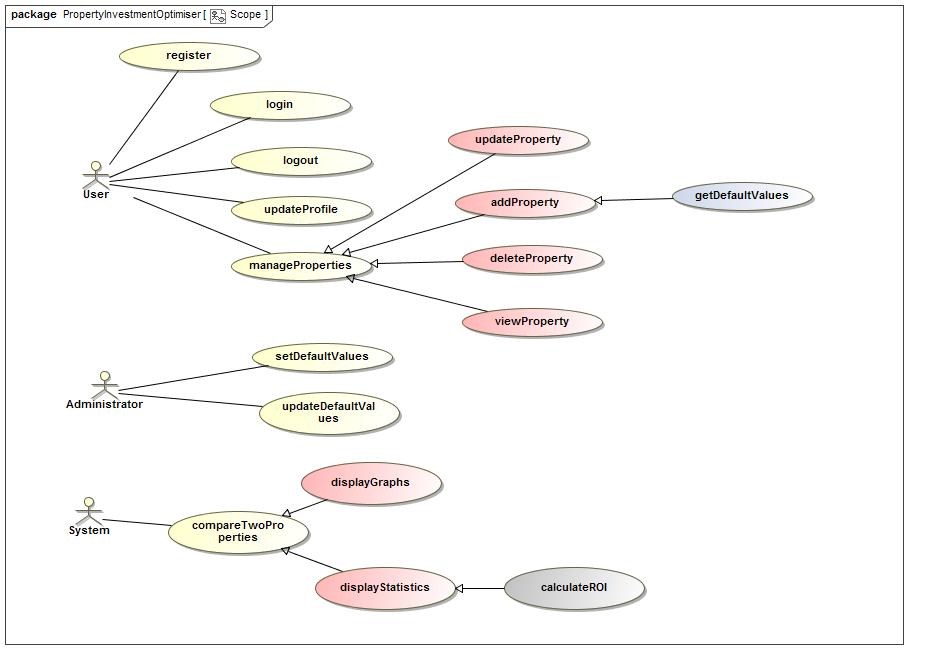
\includegraphics[width=1\textwidth]{./Image/Scope.png}
%Kudzai's Section (Vision and Background) - Stop
\newpage
\section{Software Architecture}
\subsection{Architecture requirements}
%Kudzai's Section (Architectural Scope and Quality requirements) - Start
\subsubsection{Architectural scope}
The project will be implemeneted using the Model View Controller, MVC, strucutural pattern.
The system will consist of:\begin{itemize}
	\item A website that the user will interact with in order to use the system.
	\item A database that will be used to persist objects that need to be saved.
	\item A server that will deal with the process execution and calculations of the system.
	\item A notification system that will be used to notify the user of important information that concerns them.
\end{itemize}
\subsubsection{Quality requirements}
	\begin{itemize}
		\item{\bfseries \underline{Flexibility}}\\[0.4cm]
		The system must be be able to be accessed  by more than one access channel, mainly via a computer and a 		 		smartphone. It must also not be locked to any one persistence technology. We will be using MongoDB as our persistence 			infrastructure.
		
		\item{\bfseries \underline{Maintainability}}\\[0.4cm]
		The system will be implemented with the Model View Controller structural pattern, which allows for modularisation. This 			allows the different components of the system to be maintained independently of each other. Ember.js, a 					widely-used technology with extensive support, will be used to implement MVC.
		
		\item{\bfseries \underline{Scalability}}\\[0.4cm]
		The system must be able to support as many users as possible since it is a website that will be available to a very large 			audience. Enterprise Java Beans (EJB) will be used because it can be used to develop scalable and robust enterprise 			level applications.
		
		\item{\bfseries \underline{Reliability}}\\[0.4cm]
		The webiste must have as little downtime as possible, and must display correct and accurate information at all times.
		
		\item{\bfseries \underline{Usability}}\\[0.4cm]
		Users of the system must find it very easy and intuitive to use, even to users without extnsive computer literacy. The 			system must be as efficient as possible. This will be done by implementing the latest trends in website user interface 			design.
		
		\item{\bfseries \underline{Performance}}\\[0.4cm]
		The system must execute processes smoothly between users' actions and the website, along with the graphs and 			statisitcs it will provide, must respond in a reasonble amount of time.
		
		\item{\bfseries \underline{Security}}\\[0.4cm]
		There must be no direct manipulation of the database and the server. Users will be required to login or register to be 			able to use the system. The database will be backed up to a CSV file.
		
		\item{\bfseries \underline{Auditability}}\\[0.4cm]
		Users' activities must be logged for reporting purposes.
		
		\item{\bfseries \underline{Testability}}\\[0.4cm]
		The system must be tested to ensure that each of its components are working properly. Each service contract must 			meet its pre-conditions and post-conditions. Unit and integration tests will be used to this end.
		
		\item{\bfseries \underline{Integrability}}\\[0.4cm]
		All the MVC components must be independent of each other so that they can be developed separately and integrated 			smoothly if any one of them are changed.
\end{itemize}

%Kudzai's Section (Architectural Scope and Quality requirements) - End
%Priscilla's Section (Integration and Access Channel Requirements) - Start
\subsubsection{Integration and access channel requirements}
	\begin{itemize}
		\item{\bfseries \underline{Integration}}
		\begin{itemize}
           		\item Logging into the system is done over a HTTPS POST method.
			\item The user's login details are kept in an HTTP session so the user does not need to log in everytime he/she 					makes a request to the server.
			\item The HTTPS sessions are invalidated when the user terminates his/her session by logging out.
			\item Communication between the server (back-end) and the webpage (front-end) will be facilitated by the REST 					method which uses JSON objects and HTTPS methods to send requests and get responses.
			\item The "Create, Read, Update and Delete" or CRUD actions that will make changes to the databse will be 					logged automatically. This will ensure auditability of the system. 
		\end{itemize}

		\item{\bfseries \underline{Human Access Channel}}
			\begin{itemize}
				\item End-users interact with the Web client to display the required information and do desired actions. 
			\end{itemize}

		\item{\bfseries \underline{System Access Channel}}
			\begin{itemize}
				\item The Web-based component of the system will be implememted in "Ember.js" which utilises JavaScript, HTML and "Handlebar.js".  
			\end{itemize}
	\end{itemize}
%Priscilla's Section - End
% Diana's Section - start 
\subsubsection{Architectural constraints}
	\begin{itemize}
		\item User
			\begin{itemize}
				\item Has to be registered and his/her details in the system inorder to login and be able to use the system
			\end{itemize}
		\item Time
			\begin{itemize}
				\item If a user is logged in and remains inactive for more than 30mins the user will have to login again before they can use the system again
			\end{itemize}
	\end{itemize}	
% Diana's Section - end 

% Diana's Section - start 
\subsection{Architectural patterns or styles}
\textbf{MVC (\textit{Model View Controller})}\\
Allows the system's states to change and it encapsulates the interactions
from the user and transforms these intercations into business logic.\\
\textsc{Reason:}
	\begin{itemize}
		\item Reduce presentation layers complexity and  improves flexibility
			\begin{itemize}
				\item Separates responsibilities
					\begin{itemize}
						\item Provide view onto information -\textbf{\textit{ View}}
						\item React to user events - \textbf{\textit{Controller}}
						\item Provide business services  and data - \textbf{\textit{Model}}
					\end{itemize}
				\item Allows each component to change independently
			\end{itemize}
		\item Full decoupling
			\begin{itemize}
				\item Model from both \textit{view} and \textit{controller}
			\end{itemize}
		\item Simplification
			\begin{itemize}
				\item Through separation of concerns
			\end{itemize}
		\item Reuse
			\begin{itemize}
				\item \textit{Model} components and \textit{View} components 
			\end{itemize}
		\item Maintainability
			\begin{itemize}
				\item Different components can be used, developed and maintained by different memebers of a team 
					\begin{itemize}
						\item \textit{Model} - backened developers
						\item \textit{View} - UI designers
						\item \textit{Controller} - Front-end developers
					\end{itemize}
			\end{itemize}
		\item Improved Testability
			\begin{itemize}
				\item Model/business services tested independently of UI
				\item UI tested with mock model
			\end{itemize}
	\end{itemize}

%Diana's Section  - end

\subsection{Architectural tactics or strategies}
%Sandile's Section Start
\subsection{Use of reference architectures and frameworks}
\begin{itemize}

\item JavaEE
	\begin{itemize}
		\item JavaEE contains most of the frameworks and technologies we need to develope and deploy our system.
	\end{itemize}
\end{itemize}
%Sandile's Section End

%Priscilla's Section (Access and Integration Channel Requirements) - Start
\subsection{Access and integration channels}
	\begin{itemize}
		\item This is a stand-alone application and therefore will not use other applications for all the required functionality.
		\item Plug-ins and APIs will be included, and will therefore be integrated with the main application to add specialised 				functionality. 
	\end{itemize}
%Priscilla's Section - End

%Sandile's Section Start
\subsection{Technologies}

\begin{itemize}
	\item \textit{HTML5 : }It will be used to create the front end of the system
\end{itemize}
\begin{itemize}
	\item \textit{Javascript :} front end to verify the log in details for each user it will keep track of the user logged in.
\end{itemize}
\begin{itemize}
	\item \textit{JPA:} It will be used to manage the relational data in JavaEE
\end{itemize}
\begin{itemize}
	\item \textit{EJBs:} It will be used to manage concurrency control in the system
\end{itemize}
\begin{itemize}
	\item \textit{Ember.js:} To implement the MVC patten
\end{itemize}

\begin{itemize}
	\item \textit{CSS:} It will be used for the styling of the web page
\end{itemize}
\begin{itemize}
	\item \textit{Bootsrap:} It will be used for the styling of the web page 
\end{itemize}
\begin{itemize}
	\item \textit{Web browsers:} Any web browser that supports HTML 5
\end{itemize}
%Sandile's Section End

\newpage
\section{Design overview}
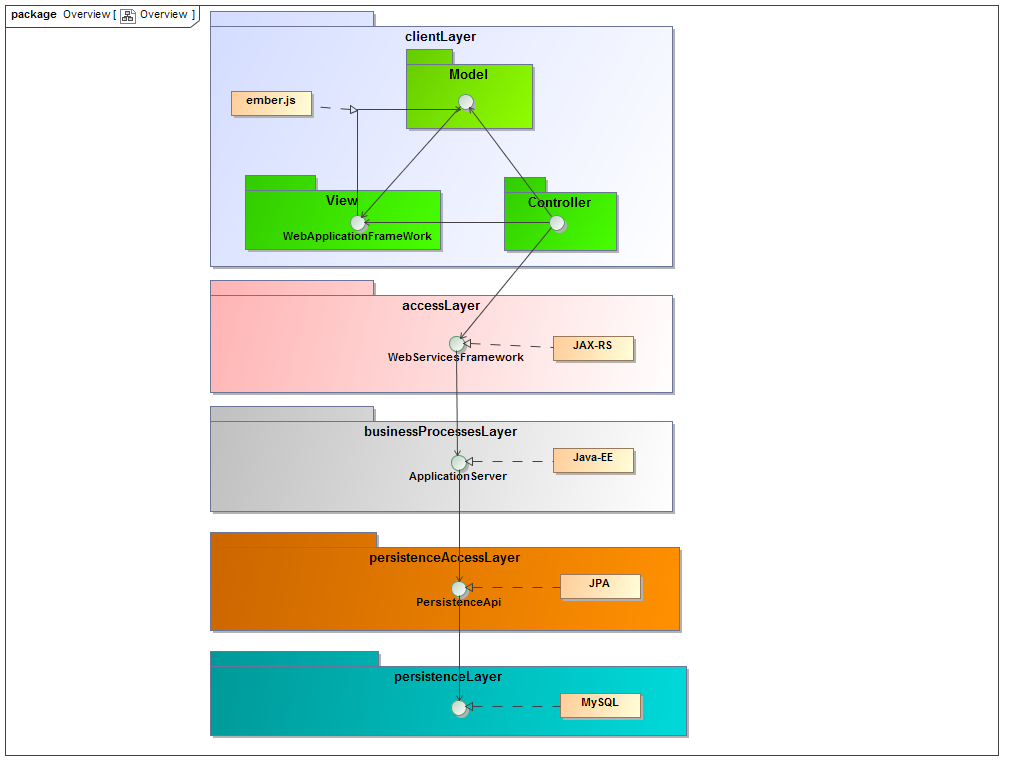
\includegraphics[width=1\textwidth]{./Image/Overview.png}



\end{document}

